\documentclass{article}
\usepackage[utf8]{inputenc}
\usepackage{amsmath, amssymb, amsthm}
\usepackage{tikz}
\usepackage{pgfplots}
\usepackage{xcolor}
\usepackage{graphicx}
\usepackage{pgf-pie}

\definecolor{background}{HTML}{2E2E2E}
\definecolor{foreground}{HTML}{E0E0E0}
\definecolor{accent}{HTML}{388E1C}
\definecolor{accent2}{HTML}{FFC300}

\pagecolor{background}
\color{foreground}

\pgfplotsset{compat=1.17}
\pgfplotsset{
	every axis/.append style={
		axis line style={color=foreground},
		tick label style={color=foreground},
		label style={color=foreground},
		legend style={fill=none, draw=foreground, text=foreground},
		major grid style={style=dotted, color=gray},
		minor grid style={style=dotted, color=gray!60}
	},
	every tick/.append style={color=foreground},
	every axis label/.append style={color=foreground},
}

\title{Mathematics Behind Economics and Finance: A Focus on the Stock Market}
\author{Badger Code}
\date{\today}

\begin{document}

\maketitle

\begin{abstract}
	This paper explores the mathematical foundations of economics and finance, with a particular focus on the stock market. By examining key concepts such as compound interest, stock valuation, and portfolio optimization, we aim to provide a comprehensive overview of the mathematical tools used in financial analysis. Visual aids, including pie charts and graphs, are incorporated to enhance understanding.
\end{abstract}

\section{Introduction}
Economics and finance are deeply intertwined with mathematics, providing a framework for understanding and predicting market behaviors. The stock market, in particular, is a complex system influenced by various economic factors. This paper delves into the mathematical principles that underpin financial theories and practices, focusing on the stock market.

\section{Mathematical Foundations of Finance}
\subsection{Compound Interest}
Compound interest is a fundamental concept in finance, representing the interest on a loan or deposit calculated based on both the initial principal and the accumulated interest from previous periods.

\[
A = P \left(1 + \frac{r}{n}\right)^{nt}
\]

Where:
\begin{itemize}
	\item $A$ is the amount of money accumulated after $n$ years, including interest.
	\item $P$ is the principal amount (the initial sum of money).
	\item $r$ is the annual interest rate (decimal).
	\item $n$ is the number of times that interest is compounded per year.
	\item $t$ is the time the money is invested for, in years.
\end{itemize}

This formula is pivotal in understanding the growth of investments over time, illustrating the exponential growth nature of compound interest.

\subsection{Stock Valuation}
Valuing stocks accurately is crucial for making informed investment decisions. The Gordon Growth Model (GGM) is one method used for this purpose:

\[
P_0 = \frac{D_0 (1 + g)}{r - g}
\]

Where:
\begin{itemize}
	\item $P_0$ is the current stock price.
	\item $D_0$ is the most recent dividend paid.
	\item $g$ is the growth rate of dividends.
	\item $r$ is the required rate of return.
\end{itemize}

The GGM assumes that dividends will continue to grow at a constant rate indefinitely, making it a useful tool for valuing mature companies with stable dividend growth.

\subsection{Portfolio Optimization}
The goal of portfolio optimization is to maximize returns for a given level of risk. The Markowitz Efficient Frontier is a key concept in this area, illustrating the set of optimal portfolios that offer the highest expected return for a defined level of risk.

The optimization problem can be formulated as follows:

\[
\min_{\mathbf{w}} \mathbf{w}^T \Sigma \mathbf{w} \quad \text{subject to} \quad \mathbf{w}^T \mathbf{1} = 1 \quad \text{and} \quad \mathbf{w}^T \mathbf{r} = R
\]

Where:
\begin{itemize}
	\item $\mathbf{w}$ is the vector of portfolio weights.
	\item $\Sigma$ is the covariance matrix of asset returns.
	\item $\mathbf{1}$ is a vector of ones.
	\item $\mathbf{r}$ is the vector of expected returns.
	\item $R$ is the target return.
\end{itemize}

This quadratic optimization problem can be solved using various numerical methods, providing investors with a strategy for selecting the best combination of assets.

\section{Visualizing Financial Data}

\subsection{Pie Chart of Portfolio Allocation}
\begin{figure}[h!]
	\centering
	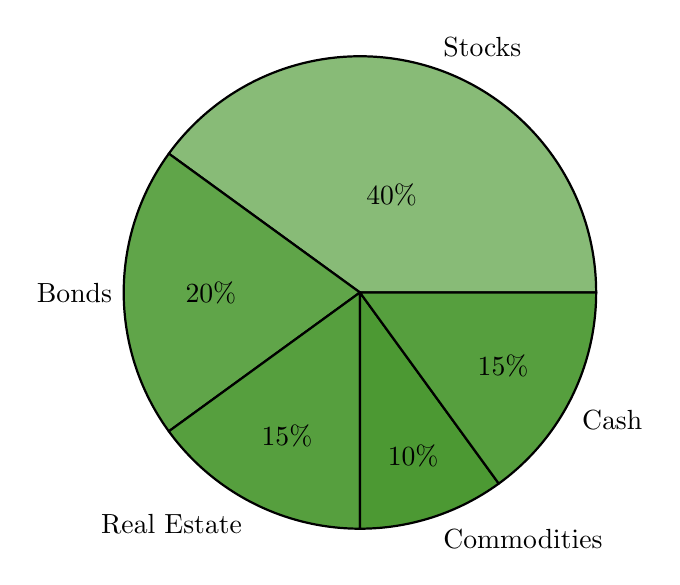
\begin{tikzpicture}
		\pie[color={accent!60, accent!80, accent!85, accent!90, accent!85}]{
			40/Stocks, 20/Bonds, 15/Real Estate, 10/Commodities, 15/Cash
		}
	\end{tikzpicture}
	\caption{Portfolio Allocation}
\end{figure}

This pie chart illustrates a diversified investment portfolio, showing the percentage allocation in different asset classes.

\subsection{Stock Market Trends}
\begin{figure}[h!]
	\centering
	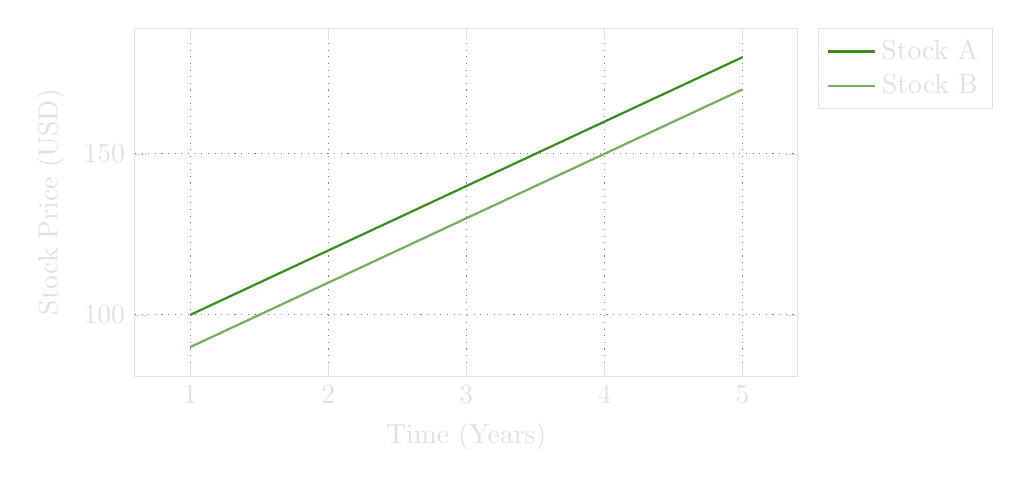
\begin{tikzpicture}
		\begin{axis}[
			width=10cm, height=6cm,
			xlabel={Time (Years)},
			ylabel={Stock Price (USD)},
			grid=major,
			legend pos=outer north east
		]
			\addplot[color=accent, thick] coordinates {
				(1, 100)(2, 120)(3, 140)(4, 160)(5, 180)
			};
			\addlegendentry{Stock A}
			
			\addplot[color=accent!70, thick] coordinates {
				(1, 90)(2, 110)(3, 130)(4, 150)(5, 170)
			};
			\addlegendentry{Stock B}
		\end{axis}
	\end{tikzpicture}
	\caption{Stock Market Trends Over 5 Years}
\end{figure}

This line graph shows the price trends of two hypothetical stocks over a five-year period, highlighting the overall growth in stock prices.

\section{Conclusion}
The mathematics of economics and finance provides powerful tools for analyzing and predicting market behaviors. Understanding concepts such as compound interest, stock valuation, and portfolio optimization is essential for making informed financial decisions. Through visualizations like pie charts and graphs, complex data can be presented in a more accessible and insightful manner.

\end{document}